\documentclass[10pt,twocolumn,a4paper]{article}
\usepackage[margin=1.8cm]{geometry}
\usepackage{booktabs,graphicx,subcaption,siunitx,hyperref,microtype,xcolor}
\usepackage{caption}
\captionsetup{font=small,labelfont=bf}

\title{\textbf{Partitioned Hash Join with Duplicates}\\\large An OpenMP Study}
\author{Gabriele Marsili \\ SPM a.y.\ 2025/26}
\date{}

\begin{document}
\maketitle
\thispagestyle{empty}

%---------------------------------------------------------------
\section{Introduction}
%---------------------------------------------------------------
This report covers the OpenMP version of the partitioned hash join
designed in Module~2. The algorithm itself is unchanged: $R$ and $S$
are partitioned on a common key mapping and an independent local join
is run on each partition. The aim here is to understand which OpenMP
constructs are actually appropriate for this kind of computation, both
on a balanced workload and on a deliberately skewed one. The C++
\texttt{std::thread} implementation from Module~2 stays in the picture
as a reference, since comparing the two runtime models is half the
point of the module.

There are two parallel variants. The first one uses loop-level
parallelism with a \texttt{parallel for} on the join phase. The second
emits explicit tasks in Longest-Processing-Time order. Both share the
same partitioning code, so the comparison between them is fair. All
experiments ran on a node of the SPM cluster.

%---------------------------------------------------------------
\section{Algorithm and OpenMP Strategies}
%---------------------------------------------------------------

\subsection{Three-phase Structure}
Given relations $R$ and $S$ with $N_R$ and $N_S$ tuples, each tuple
carries a key $k$ that is mapped to partition
$p = k \bmod P$ with $P=128$. Since $P$ is a power of two the cheaper
bitmask form $k\,\&\,(P-1)$ is used in the code. The algorithm runs
three phases on each relation in turn:

\begin{enumerate}
  \item \textbf{Histogram} -- count tuples per partition.
  \item \textbf{Scatter} -- prefix-sum offsets, then radix-write tuples
        into contiguous per-partition buffers.
  \item \textbf{Join} -- on each partition $p$, build a hash table on
        $R_p$ and probe it with every tuple of $S_p$.
\end{enumerate}

The hash table is a small flat probing structure (\texttt{FlatCountMap})
that counts duplicates incrementally during build and accumulates match
multiplicities at probe time. The flat layout with a sentinel slot
value was preferred over \texttt{std::unordered\_multimap}: it lives on
the stack, has no per-node allocations, and the ratio
\(\text{capacity}/|R_p|\approx 1.5\) keeps probing chains short.

\subsection{Loop-level Variant}
The loop variant follows the canonical \texttt{parallel for} pattern.
Each thread accumulates a private histogram in a 64-byte aligned
array, and a single thread takes care of the merge plus exclusive
prefix sum inside an \texttt{\#pragma omp single} block. The scatter
is also a \texttt{parallel for} with \texttt{schedule(static)} since
the per-tuple work is constant. The join phase is the interesting
one:

\small\begin{verbatim}
#pragma omp parallel for schedule(dynamic,1) \
    reduction(+: join_count, c1, c2)
for (uint32_t p = 0; p < P; ++p)
    join_one_partition(R[p], S[p], ...);
\end{verbatim}\normalsize

\texttt{dynamic,1} was chosen because under the skewed workload the
four hot partitions cost roughly $290\times$ more than each cold one,
and a \texttt{static} mapping would pile most of the work on whichever
threads happened to receive them. The native
\texttt{reduction(+:\dots)} clause is enough here since only three
\texttt{uint64\_t} scalars are reduced.

\subsection{Task Variant with LPT}
The task variant keeps the same histogram and scatter, but the join is
replaced by an explicit task loop:

\small\begin{verbatim}
#pragma omp parallel default(none) \
        shared(P,order,R,S,thr_results)
{
  #pragma omp single nowait
  for (uint32_t i = 0; i < P; ++i) {
    uint32_t pid = order[i];
    #pragma omp task firstprivate(pid) \
            shared(R, S, thr_results)
    { ... }
  }
}
\end{verbatim}\normalsize

The \texttt{nowait} is not decorative: without it the $T-1$ workers
would queue at the implicit barrier of \texttt{single} instead of
draining the task pool while the master is still emitting. A small
empirical detail confirmed it: removing the \texttt{nowait} added
$\sim$3\% to total time at $T=16$ on the skewed input.

The crucial ingredient is the \texttt{order} array. Before submission,
partitions are sorted in \emph{descending} order of the proxy cost
$|R_p| + |S_p|$. This is Longest Processing Time First, a classical
makespan-minimising heuristic. The sum (rather than product) is the
right proxy because hash join is linear in $|R_p|+|S_p|$, not
quadratic like a nested-loop join. Heaviest partitions enter the queue
early, so they are the first to be picked up and they have the most
threads available to absorb them.

The tasks are \emph{tied} (the default). \texttt{untied} would not
work here: the task body calls \texttt{omp\_get\_thread\_num()} to
index into the per-thread accumulator array, and an untied task could
resume on a different thread and clobber another slot.

For the reduction a manual padded array
\texttt{PaddedResult thr\_results[T]} is used, with
\texttt{alignas(64)} and a \texttt{static\_assert} that the size is
exactly one cache line. OpenMP~5.0 offers
\texttt{taskgroup task\_reduction(+:\dots)} with
\texttt{task in\_reduction(\dots)} as a more concise alternative; the
production code stays within OpenMP~4.5 because the padded array
makes the anti-false-sharing pattern explicit and is portable to the
cluster toolchain without enabling additional language levels. The same
reasoning rules out \texttt{taskloop}: it would have automatically
chunked the iteration space, breaking the LPT order.

\subsection{Synchronisation and Memory Layout}
Phase boundaries rely on the implicit barriers at the end of each
worksharing construct, with one explicit \texttt{\#pragma omp barrier}
right after the per-thread initialisation. That barrier is necessary
because \texttt{local\_hists[tid].assign(P,0)} happens outside any
worksharing region. All shared structures sit on cache-line boundaries
to avoid false sharing on the histogram and the accumulator arrays.

%---------------------------------------------------------------
\section{Skewed Workload}
%---------------------------------------------------------------
The skewed dataset is generated by a small mixture model. With
probability $\rho=0.9$ the next key is drawn from a hot pool of $H=4$
keys that are pre-selected to fall on four distinct partitions; with
probability $1-\rho=0.1$ the key is uniform on $[0,\textit{max\_key})$.
The expected fraction of records in any one hot partition is therefore
\[
  f_{\text{hot}} = \frac{\rho}{H} + \frac{1-\rho}{P}
                 = \frac{0.9}{4} + \frac{0.1}{128}
                 \approx 0.226
\]
and a cold one gets roughly $f_{\text{cold}}\approx 0.00078$, so the
ratio between hot and cold is about $290\times$.

The generator uses a deterministic \texttt{splitmix64} RNG with the
seed exposed on the CLI, so runs are reproducible bit-by-bit. The
\texttt{hot\_count} parameter is clamped to~$P$ to avoid an infinite
loop if the user asks for more hot partitions than exist (a small
guard added after triggering it during early testing).

%---------------------------------------------------------------
\section{Validation}
%---------------------------------------------------------------
The script \texttt{scripts/validate.sh} sweeps modes $\times$ workloads
$\times$ thread counts $\in\{1,2,4,8,16\}$ and compares the triple
$(\text{join\_count},\text{checksum}_1,\text{checksum}_2)$ against a
reference. For uniform the reference is the sequential baseline; for
skewed it is the parallel run at $T=1$ in the same mode. As an extra
check, loop and task at $T=4$ must produce identical triples.

The checksums are deterministic on purpose: each match contributes
$\texttt{splitmix64}(k)\cdot m$ added in $\bmod\,2^{64}$, so the result
is independent of the order in which tasks complete. All combinations
pass on the cluster.

%---------------------------------------------------------------
\section{Experimental Evaluation}
%---------------------------------------------------------------

\subsection{Setup}
The experiments run on one node of \textit{spmcluster}: dual-socket
Intel Xeon E5-2650~v3 at 2.30~GHz, 10 cores per socket, 2 hardware
threads per core (40 logical CPUs but 20 physical cores), 128~GB RAM,
two NUMA nodes. The build uses GCC~12.2 with OpenMP 4.5,
\texttt{-O3 -march=native}. Unless noted otherwise the parameters are
$N_R = 10^7$, $N_S = 2\cdot 10^7$, $P=128$, seed $42$. Every cell is
the mean of three repetitions. Affinity is fixed via
\texttt{OMP\_PROC\_BIND=close} and \texttt{OMP\_PLACES=cores}.

\subsection{Strong Scaling}
Figure~\ref{fig:strong} shows the speedup at
$T \in \{1,2,4,8,16,20,32\}$, covering the full physical-core range
of the node ($T=20$) and one operating point in the SMT range
($T=32$). The exact times are in Table~\ref{tab:strong}.

\begin{table}[t]
\centering\small
\setlength{\tabcolsep}{4pt}
\begin{tabular}{rcccc}
\toprule
$T$ & loop unif. & task unif. & loop skew & task skew \\
\midrule
1  & 0.768 & 0.759 & 0.414 & 0.413 \\
2  & 0.385 & 0.383 & 0.211 & 0.208 \\
4  & 0.245 & 0.240 & 0.140 & 0.120 \\
8  & 0.131 & 0.130 & 0.097 & 0.087 \\
16 & 0.085 & 0.084 & 0.088 & 0.085 \\
20 & 0.078 & 0.078 & 0.088 & 0.084 \\
32 & 0.076 & 0.075 & 0.089 & 0.086 \\
\bottomrule
\end{tabular}
\caption{Mean total time [s], $N_R{=}10^7$, $N_S{=}2\cdot10^7$,
         $P{=}128$.}
\label{tab:strong}
\end{table}

\begin{figure}[t]
\centering
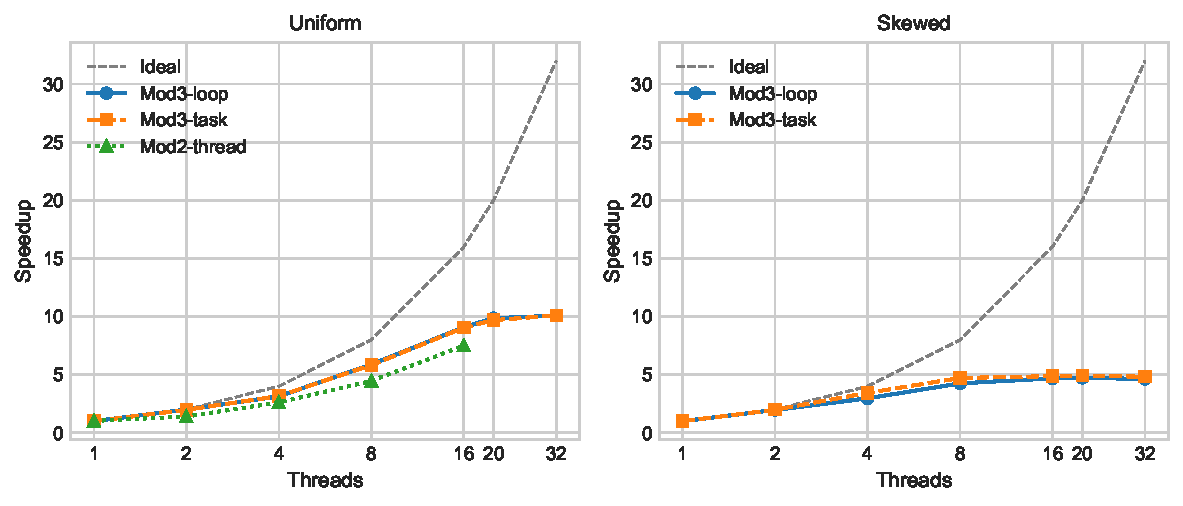
\includegraphics[width=\columnwidth]{fig_strong.pdf}
\caption{Strong scaling. Speedup is $T(1)/T(p)$ averaged over three
repetitions. The dashed line is the ideal.}
\label{fig:strong}
\end{figure}

On uniform input the two variants are essentially indistinguishable
(within $\sim$1\%): the workload is already balanced and there is no
room for the LPT ordering to help. Speedup grows almost linearly up to
$T=8$ ($\sim 5.85\times$, efficiency $73\%$). At $T=16$ both variants
sit around $9.1\times$; at $T=20$, where all physical cores are used,
the speedup reaches $\sim 9.7\times$ (efficiency $48.5\%$). Past
$T=20$, the extra threads share physical cores via SMT, and the
speedup grows only marginally to $\sim 10.1\times$ at $T=32$. This is
the expected behaviour for a memory-bound kernel: SMT helps with
latency hiding but does not double the available cache bandwidth.

The skewed case is where the two strategies separate. At $T=4$ the
task variant takes $0.120$~s versus $0.140$~s for the loop, a
$\sim$14\% advantage that comes purely from emitting the four hot
partitions first; at $T=8$ the gap is still around $11\%$. From $T=8$
onwards the time barely decreases for either variant: four hot
partitions cannot keep sixteen, twenty or thirty-two threads busy, no
matter the schedule. The skewed efficiency at $T=20$ is only
$\sim 24\%$, a frank reminder that LPT softens skew but does not
remove it.

\subsection{Weak Scaling}
$N_R$ scales proportionally with $T$ ($2{\cdot}10^6$ tuples per
thread), see Figure~\ref{fig:weak}.

\begin{figure}[t]
\centering
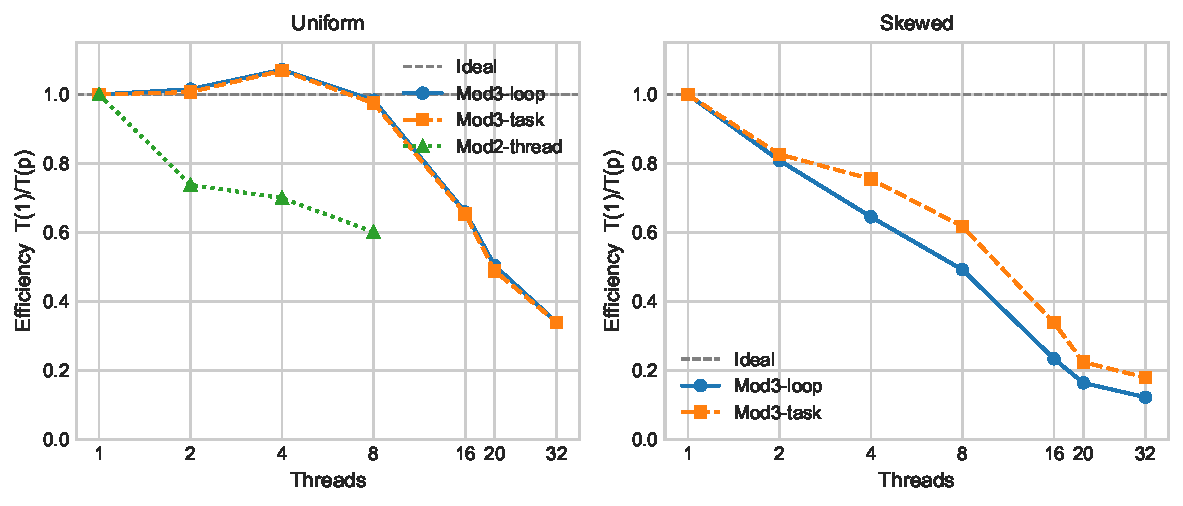
\includegraphics[width=\columnwidth]{fig_weak.pdf}
\caption{Weak scaling. Efficiency is $T(1)/T(p)$ with the input scaled
linearly with the thread count.}
\label{fig:weak}
\end{figure}

Uniform weak scaling holds reasonably well up to one full socket:
total time grows from $0.179$~s at $T=1$ to $0.197$~s at $T=8$
(efficiency $\sim 91\%$), then degrades to $\sim 73\%$ at $T=16$ once
both sockets are involved. Memory bandwidth is the limiting factor:
the scatter phase reads and writes a $1$~GB working set linearly with
$T$, and the dual-socket aggregate bandwidth saturates before the
core count does. Skewed weak scaling, by contrast, falls off a cliff:
doubling $N_R$ also doubles the load on the four hot partitions, so
they remain the bottleneck and grow proportionally with the input.
At $T=16$ skewed efficiency is around $22\%$.

\subsection{Phase Breakdown}
The breakdown in Figure~\ref{fig:breakdown} confirms what one would
expect from a memory-bound algorithm: scatter $S$ is the most
expensive single phase under uniform input (about 30--33\% of the
total), followed by the join. On skewed input the picture rotates: as
$T$ grows, hist and scatter shrink almost ideally because the
per-tuple work is partition-blind, but the join keeps growing
relatively until at $T=16$ it accounts for around 65\% of the total
time. This is the visible footprint of skew on the timing.

\begin{figure}[t]
\centering
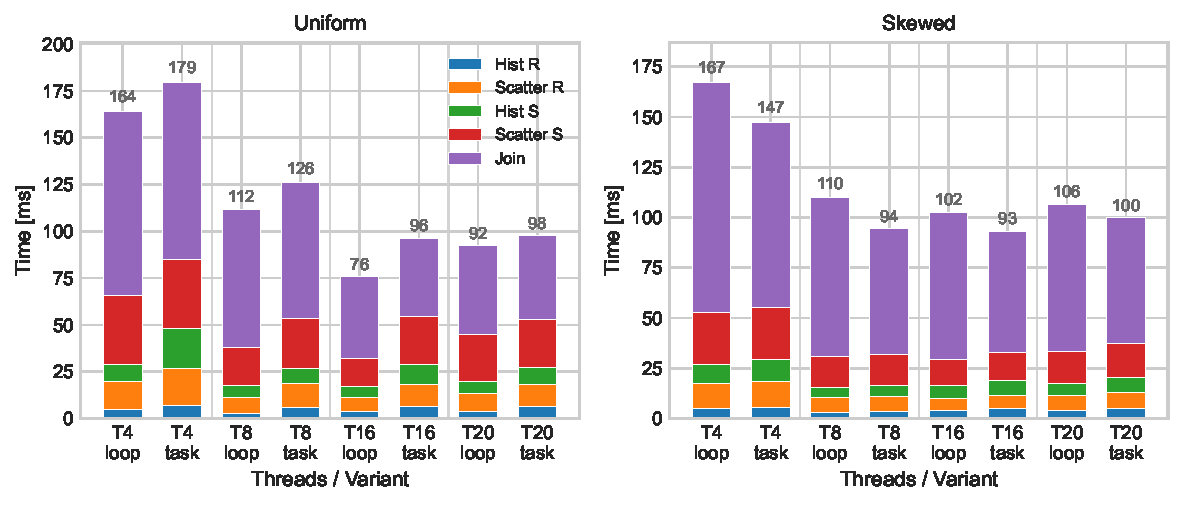
\includegraphics[width=\columnwidth]{fig_breakdown.pdf}
\caption{Phase breakdown for $T \in \{1,4,16\}$, uniform workload.
Mod3 OpenMP (loop and task) on the left, Mod2 \texttt{std::thread} on
the right.}
\label{fig:breakdown}
\end{figure}

\subsection{Schedule Sensitivity}
Figure~\ref{fig:schedule} reports the join time at $T=8$ for five
schedule policies (\texttt{static}, \texttt{static,1},
\texttt{dynamic,1}, \texttt{dynamic,4}, \texttt{guided,1}). All
policies converge within $\sim$1\%. With $P=128$ and $T=8$ the ratio
$P/T=16$ is high enough that even \texttt{static} balances the load
reasonably: each thread gets a chunk of $16$ partitions, and across
the chunk the heavy and light partitions average out. The result is
consistent with the expected behaviour of static block partitioning
when the unit of work is small relative to the per-thread quota.

\begin{figure}[t]
\centering
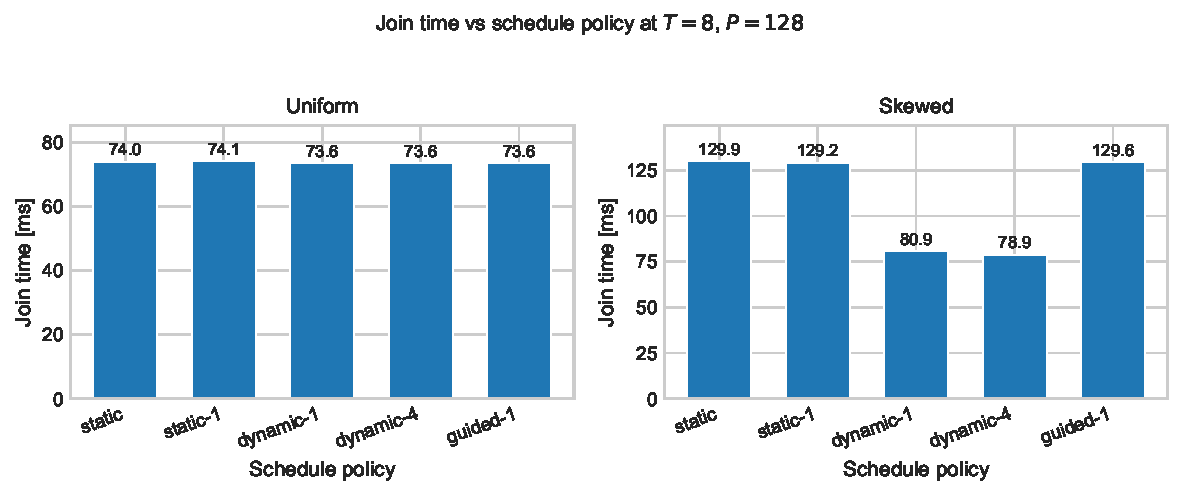
\includegraphics[width=\columnwidth]{fig_schedule.pdf}
\caption{Join time at $T=8$ across five schedule policies.}
\label{fig:schedule}
\end{figure}

The choice of \texttt{dynamic,1} as the production default is driven
not by the $T=8$ measurements but by the asymptotic behaviour at
larger $T$ and lower $P/T$ ratios: the heuristic is robust regardless
of partition-size variance, at the cost of a small runtime overhead
that is invisible at this granularity.

\subsection{Comparison with Module 2}
The Module~2 implementation uses a hand-rolled \texttt{std::thread}
pool with \texttt{BlockingQueue} stages between phases. Same
algorithm, same input, same node, but a very different runtime model.
Figure~\ref{fig:m2vsm3} plots time and speedup against $T$ for the
uniform workload across the full thread range
$T\in\{1,2,4,8,16,20,32\}$, matching the granularity used in the
Module~2 evaluation. Table~\ref{tab:m2} reports key numbers at $T=16$,
$T=20$ (full physical-core saturation), and $T=32$ (SMT range).

\begin{figure}[t]
\centering
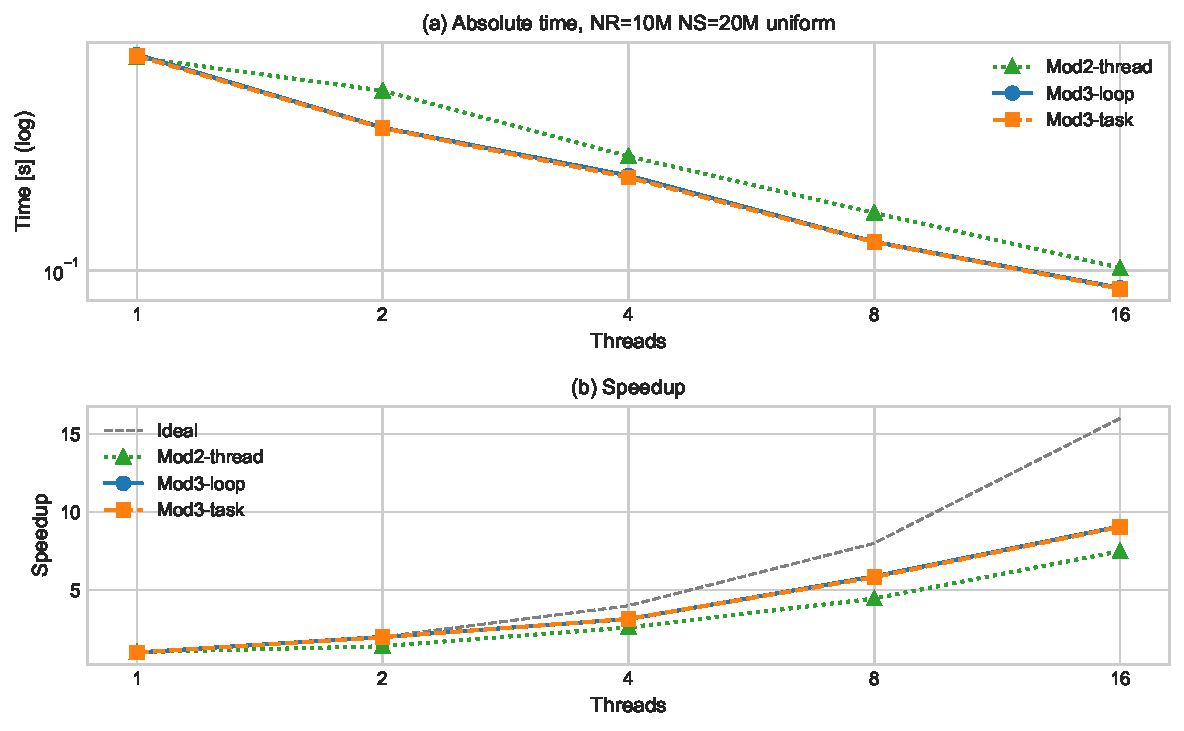
\includegraphics[width=\columnwidth]{fig_m2_vs_m3.pdf}
\caption{Module 2 \texttt{std::thread} versus Module 3 OpenMP, uniform
input.}
\label{fig:m2vsm3}
\end{figure}

\begin{table}[t]
\centering\small
\setlength{\tabcolsep}{4pt}
\begin{tabular}{lccc|ccc}
\toprule
 & \multicolumn{3}{c|}{$T(p)$ [s]} & \multicolumn{3}{c}{Speedup} \\
$T$ & Mod2 & M3 loop & M3 task & Mod2 & M3 loop & M3 task \\
\midrule
seq & \multicolumn{3}{c|}{0.767} & \multicolumn{3}{c}{1.00} \\
1  & 0.747 & 0.768 & 0.759 & 1.03 & 1.00 & 1.01 \\
2  & 0.546 & 0.385 & 0.383 & 1.40 & 2.00 & 1.98 \\
4  & 0.293 & 0.245 & 0.240 & 2.61 & 3.14 & 3.16 \\
8  & 0.172 & 0.131 & 0.130 & 4.46 & 5.87 & 5.82 \\
16 & 0.102 & 0.085 & 0.084 & 7.49 & 9.08 & 9.05 \\
20 & 0.103 & 0.078 & 0.078 & 7.41 & \textbf{9.86} & 9.69 \\
32 & 0.089 & 0.076 & 0.075 & 8.64 & 10.08 & \textbf{10.10} \\
\bottomrule
\end{tabular}
\caption{Module 2 \texttt{std::thread} vs Module 3 OpenMP, uniform
$N_R{=}10^7$, $N_S{=}2{\cdot}10^7$. The first row is the shared
sequential baseline (0.767~s, mean of 3 runs). Mod2 speedups use
$T_{\text{seq}}/T(p)$ (so $T{=}1$ shows the std::thread one-worker
overhead, $\sim$3\%); Mod3 speedups use each variant's own
$T(1)\!\approx\!T_{\text{seq}}$, which differs from $T_{\text{seq}}$
by less than $0.2\%$.}
\label{tab:m2}
\end{table}

OpenMP wins at every $T \geq 2$, and the gap widens at small thread
counts. At $T=2$ the OpenMP variants are roughly $40\%$ faster than
the \texttt{std::thread} version; at $T=20$ the gap is still around
$25\%$ in absolute time. Looking at the phase breakdowns, the
histogram phase is about $4.6\times$ faster in OpenMP at $T=8$
($3.3$~vs.~$15.2$~ms), while the memory-bound scatter and join phases
differ by only $5$--$20\%$. The runtime model accounts for the
difference: OpenMP re-uses a persistent thread pool with cheap
implicit barriers, whereas the Module~2 design pays for explicit
queue push/pop with condition variables between phases, around
$10$--$20~\mu$s of synchronisation overhead per phase per thread. On a
phase as short as a histogram over $10^7$ tuples this overhead
dominates.

A second observation comes from the SMT range. Module~2 shows a
plateau between $T=16$ and $T=20$ (time grows slightly from $0.102$
to $0.103$~s), suggesting that the queue-based synchronisation does
not scale cleanly past one full socket. OpenMP keeps improving up to
$T=20$ ($0.078$~s, $9.86\times$) and gains a further $4$\% at $T=32$
in SMT mode. The persistent pool absorbs the additional threads
without measurable contention, which is the kind of property the
runtime is engineered for.

The usual trade-off applies. Module~2 took roughly twice as much code:
the \texttt{BlockingQueue}, the worker loop, the explicit join, and
so on. Module~3 fits the same algorithm into a handful of pragmas.
When the problem does not match the canonical parallel-for or
task-pool patterns (a custom data-flow with priorities would be one
example), the explicit-threads route gives more control and is worth
the verbosity. The partitioned hash join fits OpenMP cleanly, and
OpenMP wins.

%---------------------------------------------------------------
\section{Discussion}
%---------------------------------------------------------------
On uniform input loop and task strategies behave equivalently, and
the choice between them is a matter of style. On skewed input
LPT-ordered tasks give a measurable advantage at moderate thread
counts ($T = 4$--$8$), but they cannot rescue a workload where the
hot-partition count drops below the thread count: the structural
imbalance dominates beyond that point. The schedule-policy study
shows a $\sim 1\%$ spread between the five options, which is exactly
the expected behaviour at $P/T = 16$. Across every operating point
OpenMP outperforms the Module~2 \texttt{std::thread} version, with
the gap widest at small thread counts and concentrated in the short
synchronisation-sensitive phases. At full physical-core saturation
($T=20$) OpenMP reaches $9.86\times$ speedup against the $7.41\times$
of Module~2, and continues to scale modestly into the SMT range while
Module~2 plateaus.

The main avenue left for improvement is NUMA-aware allocation of the
input relations: $R$ and $S$ are currently generated single-threaded,
which limits the weak-scaling ceiling reachable at $T \geq 16$.
Replacing the manual padded reduction array with
\texttt{task\_reduction} from OpenMP~5.0 would also shorten the code
without affecting performance, on toolchains where this language
level is enabled by default.

\end{document}
